\documentclass[11pt]{aghdpl}
% \documentclass[en,11pt]{aghdpl}  % praca w języku angielskim
\usepackage[polish]{babel}
%\usepackage[english]{babel}
\usepackage[utf8]{inputenc}
\usepackage[T1]{fontenc}

% dodatkowe pakiety
\usepackage{enumerate}
\usepackage{listings}
\lstloadlanguages{TeX}

%kolorowanie linków + działanie linków
\usepackage[colorlinks=true,urlcolor=blue,linkcolor=black,citecolor=green]{hyperref}

\usepackage{listings}
\usepackage{xcolor}
\definecolor{listinggray}{gray}{0.9}
\definecolor{lbcolor}{rgb}{0.9,0.9,0.9}
\lstset{
  backgroundcolor=\color{lbcolor},
  tabsize=4,
  language=C++,
  captionpos=b,
  tabsize=3,
  frame=lines,
  numbers=left,
  numberstyle=\tiny,
  numbersep=5pt,
  breaklines=true,
  showstringspaces=false,
  basicstyle=\footnotesize,
%  identifierstyle=\color{magenta},
  keywordstyle=\color[rgb]{0,0,1},
  commentstyle=\color{Darkgreen},
  stringstyle=\color{red}
  }
\lstset{
  literate={ą}{{\k{a}}}1
           {ć}{{\'c}}1
           {ę}{{\k{e}}}1
           {ó}{{\'o}}1
           {ń}{{\'n}}1
           {ł}{{\l{}}}1
           {ś}{{\'s}}1
           {ź}{{\'z}}1
           {ż}{{\.z}}1
           {Ą}{{\k{A}}}1
           {Ć}{{\'C}}1
           {Ę}{{\k{E}}}1
           {Ó}{{\'O}}1
           {Ń}{{\'N}}1
           {Ł}{{\L{}}}1
           {Ś}{{\'S}}1
           {Ź}{{\'Z}}1
           {Ż}{{\.Z}}1
}



%\usepackage[pdftex]{graphicx}
%---------------------------------------------------------------------------

\author{Żaneta Błaszczuk, Rafał Kozik, Filip Kubicz, Jakub Nowak, Jakub Porębski}
\shortauthor{Ż. Błaszczuk, R. Kozik, F. Kubicz, J. Nowak, J. Porębski}

\titlePL{Model skrzyżowania równorzędnego wraz z porównaniem sygnalizacji świetlnej: stałoczasowej oraz inteligentnie sterowanej }
\titleEN{Model of road intersection with two types of controlled traffic lights}

\shorttitlePL{Model skrzyżowania z sygnalizacją} % skrócona wersja tytułu jeśli jest bardzo długi
%\shorttitleEN{Thesis in \LaTeX}

\thesistype{Modelowanie układów fizycznych i biologicznych}
%\thesistype{Master of Science Thesis}

\supervisor{dr inż. Ireneusz Wochlik}

\degreeprogramme{Automatyka i Robotyka}
%\degreeprogramme{Computer Science}

\date{2014}

\department{Katedra Automatyki}
%\department{Department of Applied Computer Science}

\faculty{Wydział Elektrotechniki, Automatyki,\protect\\[-1mm] Informatyki i Inżynierii Biomedycznej}
%\faculty{Faculty of Electrical Engineering, Automatics, Computer Science and Biomedical Engineering}

\setlength{\cftsecnumwidth}{5mm}

\begin{document}
\titlepages

\section{Model skrzyżowania}
Nasz model skrzyżowania składa się z 4 dróg dojazdowych, które są kolejkami FIFO oraz z sygnalizacji świetlnej. Graficznie mogłoby ono wyglądać tak: 

\begin{figure}[h!]
	\centering
	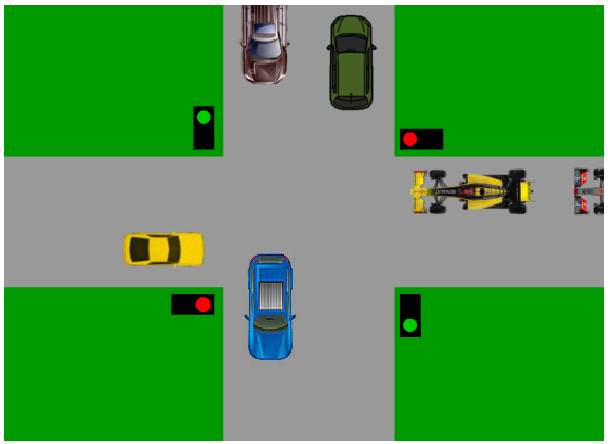
\includegraphics[width=66mm]{model.png}
	\caption{Graficzne przedstawienie modelu skrzyżowania.}	
	\label{model}
\end{figure} 

Działanie modelu polega na przepuszczaniu samochodów przez skrzyżowanie.  Pierwszy samochód z każdej z kolejek FIFO podejmuje decyzję, czy przejechać przez skrzyżowanie, czy też nie. Przejazd jest dozwolony, gdy  samochód dostaje światło zielone, a zabroniony przy świetle czerwonym.
Stan kolejek dojazdowych do skrzyżowania jest aktualizowany po każdej zmianie świateł -- model dyskretny. Liczba przybywających samochodów jest generowana losowo przez generator srand.

Skrzyżowanie posiada:
\begin{itemize}
	\item 4 drogi dojazdowe -- kolejki FIFO samochodów
	\item sygnalizację świetlną
\end{itemize}

Samochód posiada:
\begin{itemize}
	\item Czas przejazdu przez skrzyżowanie -- czas jaki zajmuje samochodowi przejechanie przez światła na tyle, że następny samochód może decydować, czy jechać, czy pozostać na światłach (czas o jaki samochód opóźnia podjęcie decyzji o przejeździe następnemu).
	Czas ten jest generowany losowo przez generator liczb losowych srand.
	\item Czas oczekiwania na przejazd -- w celu analizy jakości sterowania.
\end{itemize}

Model zaimplementowaliśmy w języku C++ wykorzystując bibliotekę STL kolejek FIFO. Staraliśmy się zrealizować symulację w ten sposób, by można było sterować wszystkimi parametrami w celu badania mechanizmu skrzyżowań z sygnalizacją świetlną. Możliwość zmiany maksymalnej ilości przybywających samochodów oraz czasu ich przebywania na skrzyżowaniu służy do modelowania natężenia ruchu oraz ,,gatunku'' kierowców.

Jednocześnie wyróżniliśmy stan ,,rozładowania'' skrzyżowania. występuje on w momencie, gdy na wszystkich drogach dojazdowych liczba samochodów jest mniejsza bądź równa maksymalnej równa liczbie samochodów, które w danej zmianie świateł mogły na skrzyżowanie przyjechać.

\section{Sygnalizacja}
Sygnalizacja świetlna posiada 2 stany, w których przepuszcza albo samochody w kierunku pionowym lub w poziomym. Każdy rodzaj sygnalizacji posiada opóźnienie spowodowane światłem pomarańczowym w czasie którego skrzyżowanie pozostaje nieczynne. Opóźnienie wpływa na zmniejszenie czasu przejazdu. W dalszych rozważaniach przyjęliśmy opóźnienie jako 2 sekundy.
Przy każdej zmianie świateł przybywa maksymalnie 5 samochodów (do każdej z kolejek), a każdy samochód przejeżdża skrzyżowanie w mniej niż 5 sekund.

Działanie skrzyżowania można zobaczyć na wykresie \ref{dzialanie}:
\begin{figure}[h!]
	\centering
	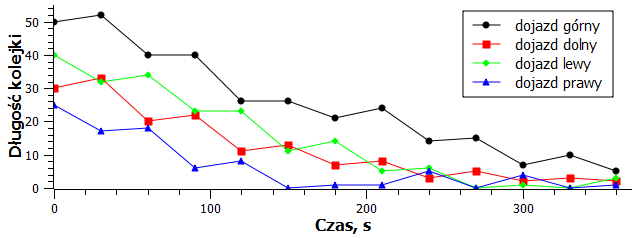
\includegraphics[width=0.80\textwidth]{dzialanie.png}
	\caption{Wykres długości kolejek samochodów w zależności od czasu.}	
	\label{dzialanie}
\end{figure}

Wykres przedstawia działanie skrzyżowania z sygnalizacją stałoczasową ustawioną na czas światła zielonego równy 30 sekund. 

Długość każdej z kolejek spada co drugi okres czasu, kiedy pojawia się światło zielone. 

\subsection{Sygnalizacja stałoczasowa}
Jest to najprostszy sposób sterowania ruchem na skrzyżowaniu. Posiada on tylko jeden parametr - czas światła zielonego. 
Wybór optymalnej wartości tego parametru dokonaliśmy testując zachowanie skrzyżowania na impuls początkowy jakim jest 100 samochodów na jednej z dróg dojazdowych. parametrem porównawczym jest tu czas obsługi samochodów przez skrzyżowanie. Decyduje on o relatywnym zadowoleniu kierowców.
\begin{figure}[h!]
	\centering
	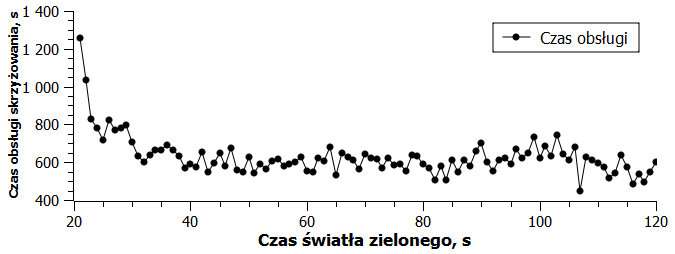
\includegraphics[height=55mm]{czasobs(time).png}
	\caption{Zależność czasu obsługi skrzyżowania od czasu światła zielonego w sygnalizacji stałoczasowej}	
	\label{czasobs(time)}
\end{figure}

Z wykresu [\ref{czasobs(time)}] wynika, że dla tych warunków czasy większe od 40 sekund pozwalają na osiągnięcie optymalnego czasu obsługi na poziomie około 600 sekund \label{600}. 

Reakcję skrzyżowania na różną liczbę początkową samochodów dla czasu światła zielonego 50 sekund obrazuje wykres [\ref{czasobs(ilosc)}]:

\begin{figure}[h!]
	\centering
	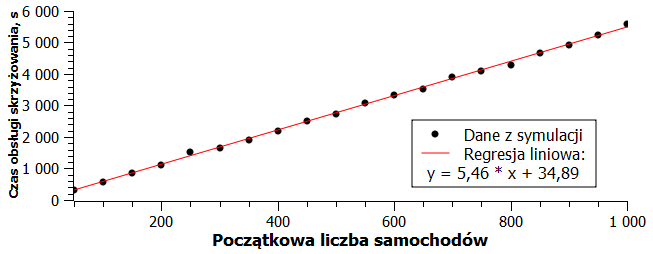
\includegraphics[height=55mm]{czasobs(ilosc).png}
	\caption{Zależność czasu obsługi skrzyżowania od ilości początkowej samochodów}	
	\label{czasobs(ilosc)}
\end{figure} 

Równanie regresji liniowej dla wykresu [\ref{czasobs(ilosc)}] to:
\begin{equation}
	 y = 5,46 * x + 34,89 \qquad \qquad \qquad R^2 = 0,999
\end{equation}

\subsection{Sygnalizacja inteligentna}
W celu zamodelowania sygnalizacji, która reaguje na dane o stanie modelu zastosowaliśmy regulator P, najprostszy nam dostępny. Uchybem regulacji jest w tym wypadku sumaryczna długość kolejek w kierunku, na którym jest aktualnie światło zielone.
Współczynnik proporcjonalności dobraliśmy doświadczalnie testując odpowiedzi układu na skok 100 samochodów w jednej z kolejek (tak samo jak w [\ref{czasobs(time)}]). Najlepsze wyniki otrzymaliśmy dla współczynnika proporcjonalności równego $2.2$, a czas oczekiwania na ,,rozładowanie'' skrzyżowania wyniósł około 250 sekund (dla sterowania stałoczasowego było to 600 sekund [\ref{600}]).

Czas obsługi skrzyżowania sterowanego przy użyciu regulatora $P$ w zależności od ilości początkowego impulsu samochodów przedstawia wykres [\ref{czasobs(ilosc)2}].

\newpage

\begin{figure}[h!]
	\centering
	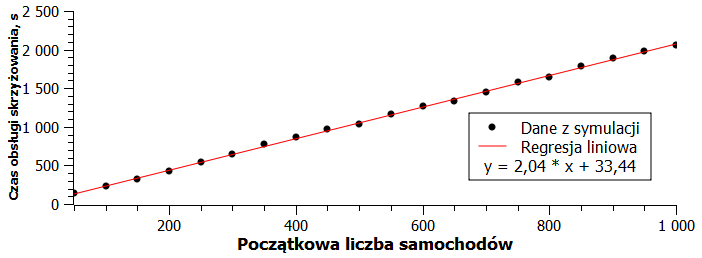
\includegraphics[height=55mm]{czasobs(ilosc)2.png}
	\caption{Zależność czasu obsługi skrzyżowania od ilości początkowej samochodów}	
	\label{czasobs(ilosc)2}
\end{figure}

Równanie regresji liniowej dla tego wykresu to:
\begin{equation}
	 y = 2,04 * x + 33,44 \qquad \qquad \qquad R^2 = 0,999 
	 \label{regresja2}
\end{equation}

Mniejszy współczynnik kierunkowy w równaniu regresji [\ref{regresja2}] świadczy o tym, że skrzyżowanie sterowane przy użyciu regulatora P jest ponad 2 razy skuteczniejsze od optymalnego sterowania stałoczasowego.

\begin{equation}
	\frac{a_{staloczasowe}}{a_{inteligentne}} = \frac{5,46}{2,04} = 2,68
\end{equation}

Jednakże sterowanie za pomocą regulatora P jest dość kontrowersyjne. Dla tych samych danych początkowych co w zaprezentowanym powyżej przykładzie działania skrzyżowania [\ref{dzialanie}] sterowanie regulatorem P wygląda tak [\ref{dzialanie2}]:
\begin{figure}[h!]
	\centering
	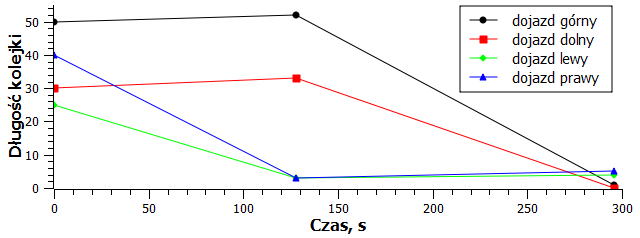
\includegraphics[height=55mm]{dzialanie2.png}
	\caption{Zależność czasu obsługi skrzyżowania od ilości początkowej samochodów}	
	\label{dzialanie2}
\end{figure}

\newpage

\section{Wnioski}
\begin{enumerate}
	\item Sterowanie skrzyżowaniem za pomocą prostego regulatora P jest ponad 2 razy szybsze od sygnalizacji stałoczasowej, chociaż jego rozwiązanie może być dość zaskakujące.
	\item Zaimplementowany model może posłużyć do bardziej  zaawansowanych symulacji prawdziwych sytuacji w ruchu ulicznym.
\end{enumerate}

\section{Bibliografia}
\begin{enumerate}
%\item Ilustracja skrzyżowania: \href{http://www.wf.gimkonst.pl/viewpage.php?page_id=50}{ www.wf.gimkonst.pl}.
\item regulator PID -- ,,Podstawy Automatyki -- wykład'' prof. Krzysztof Oprzędkiewicz.

\end{enumerate}


\end{document}